%----------------------------------------------------------------------------------------
%	Live Repository
%----------------------------------------------------------------------------------------
\chapter{Live Repository}\label{chap:live}
\lhead{\emph{Live Repository}} % Set the left side page header to "Introduction"

%\section{Summary}
In the analysis of recent secondary studies, we notice a gap of one or even two years elapses between the covered period of literature and the year the review appears. 
This is understandable, because the authors may need substantial time for analyzing the selected studies and then writing the article, followed by several months for the peer review process. 
Moreover, even if this temporal gap is reduced to a minimum, as long as the investigated topic remains active, new primary studies will always appear, soon distancing any systematic literature review (\slr) from the status of literature.  
If the purpose of an \slr is to provide an up-to-date summary of existing work on a topic, frequent updates are required to include newly appearing relevant studies.
Also, it can happen that the original research questions and findings lose relevance, or are superseded by newer results.
As previously questioned in other disciplines~\cite{Garneri3507}, Mendes et al.~\cite{MENDES2020110607} have recently investigated the issue of {\slr}s in software engineering becoming obsolete and of when and how they would need to be updated. 
Specifically, in line with~\cite{Garneri3507}, they conclude that {\slr}s should be updated based on two conditions: \textit{i)} new relevant methods, studies or information become available; or \textit{ii)} the adoption or inclusion of previous and new research cause an impact to the findings, conclusions or credibility of the original \slr.

Thus, it is inevitable that a literature review becomes outdated after some time, as new research comes out that cannot be included in the published paper, limiting the long-term value of the work, since the text will no longer reflect the ongoing research in the field.
In consideration of these challenges, rather than providing a static list of the studies found while conducting the review, along with this work we release an \textit{open and updatable repository}, which is an integral contribution of this study, and
the review from \Cref{chap:literature_review} is enhanced to become a \textit{live} systematic review\footnote{We notice that our concept of a ``live'' systematic review, while inspired by similar aims, should not be confused with the much more formalized approach for conducting \textit{living systematic reviews} recently adopted in medicine, as illustrated by \url{https://community.cochrane.org/review-production/production-resources/living-systematic-reviews}.}. 

Aggregating long-term value to this work, we have made the list of papers and the information extracted from them available as an online live repository\footnote{Available at: \url{https://renangreca.github.io/literature-repository}.}.
The papers listed in \Cref{table:selected} and discussed throughout \Cref{chap:literature_review} serve as the starting point for a bibliography that will continue to grow year over year, through updates to the review and submissions by authors.
We hope this website will serve as reference to anyone who is interested in practical applications of regression testing techniques in the coming years.

%The group of papers listed and discussed in \Cref{chap:literature_review} provide the initial contents of this live repository, which is made available online.
%Over time, through updates to the review and submissions by authors, we expect this list to grow.
 
The intent is to invite the community to contribute with newly published works with approaches to \rt that are relevant in \rea.
Additionally, it could also be incremented with works already published but that, for some reason, escaped our selection.
This will allow us to keep track of newly published studies, 
as well as recover papers that had theoretical motivations and unclear applicability, but that eventually provided benefits in practice.
At periodic intervals (planned to be once per year), we will check new results for queries and suggestions from the community and decide how to update the collection of studies.
With this, another \slr covering the same topic should not be needed within the foreseeable future.

The repository also contains a separate section for relevant literature reviews, initially populated by the reviews mentioned in \Cref{sec:lit_related}.
This provides a starting point for new researchers and a place to gather the overarching themes of the field.

%\section{The Repository}\label{sec:live_repo}
%Literature reviews provide important information to researchers starting out in a field or practitioners who are curious to know the latest innovations, but do not have time to fully explore journals and conferences.
%However, it is inevitable that a literature review such as this becomes outdated after some time, as new research comes out that cannot be included in the published paper.
%This of course limits the long-term value of the work, since the text will no longer reflect the ongoing research in the field.

\section{Implementation}\label{subsec:live_implementation}

The website is implemented using the Jekyll static website generator and the associated Liquid templating language.
The data that populates the webpages is initially extracted from the spreadsheets originally used to manage the \slr from \Cref{chap:literature_review}.
The spreadsheets are exported as CSV files, then converted to JSON files for better readability, also making it easier for each paper to have its own data file.
The fields for each paper mostly correspond to the data extraction table (\Cref{table:extraction}).
The website itself is open-source and hosted via GitHub Pages.

\begin{figure}
  \center
  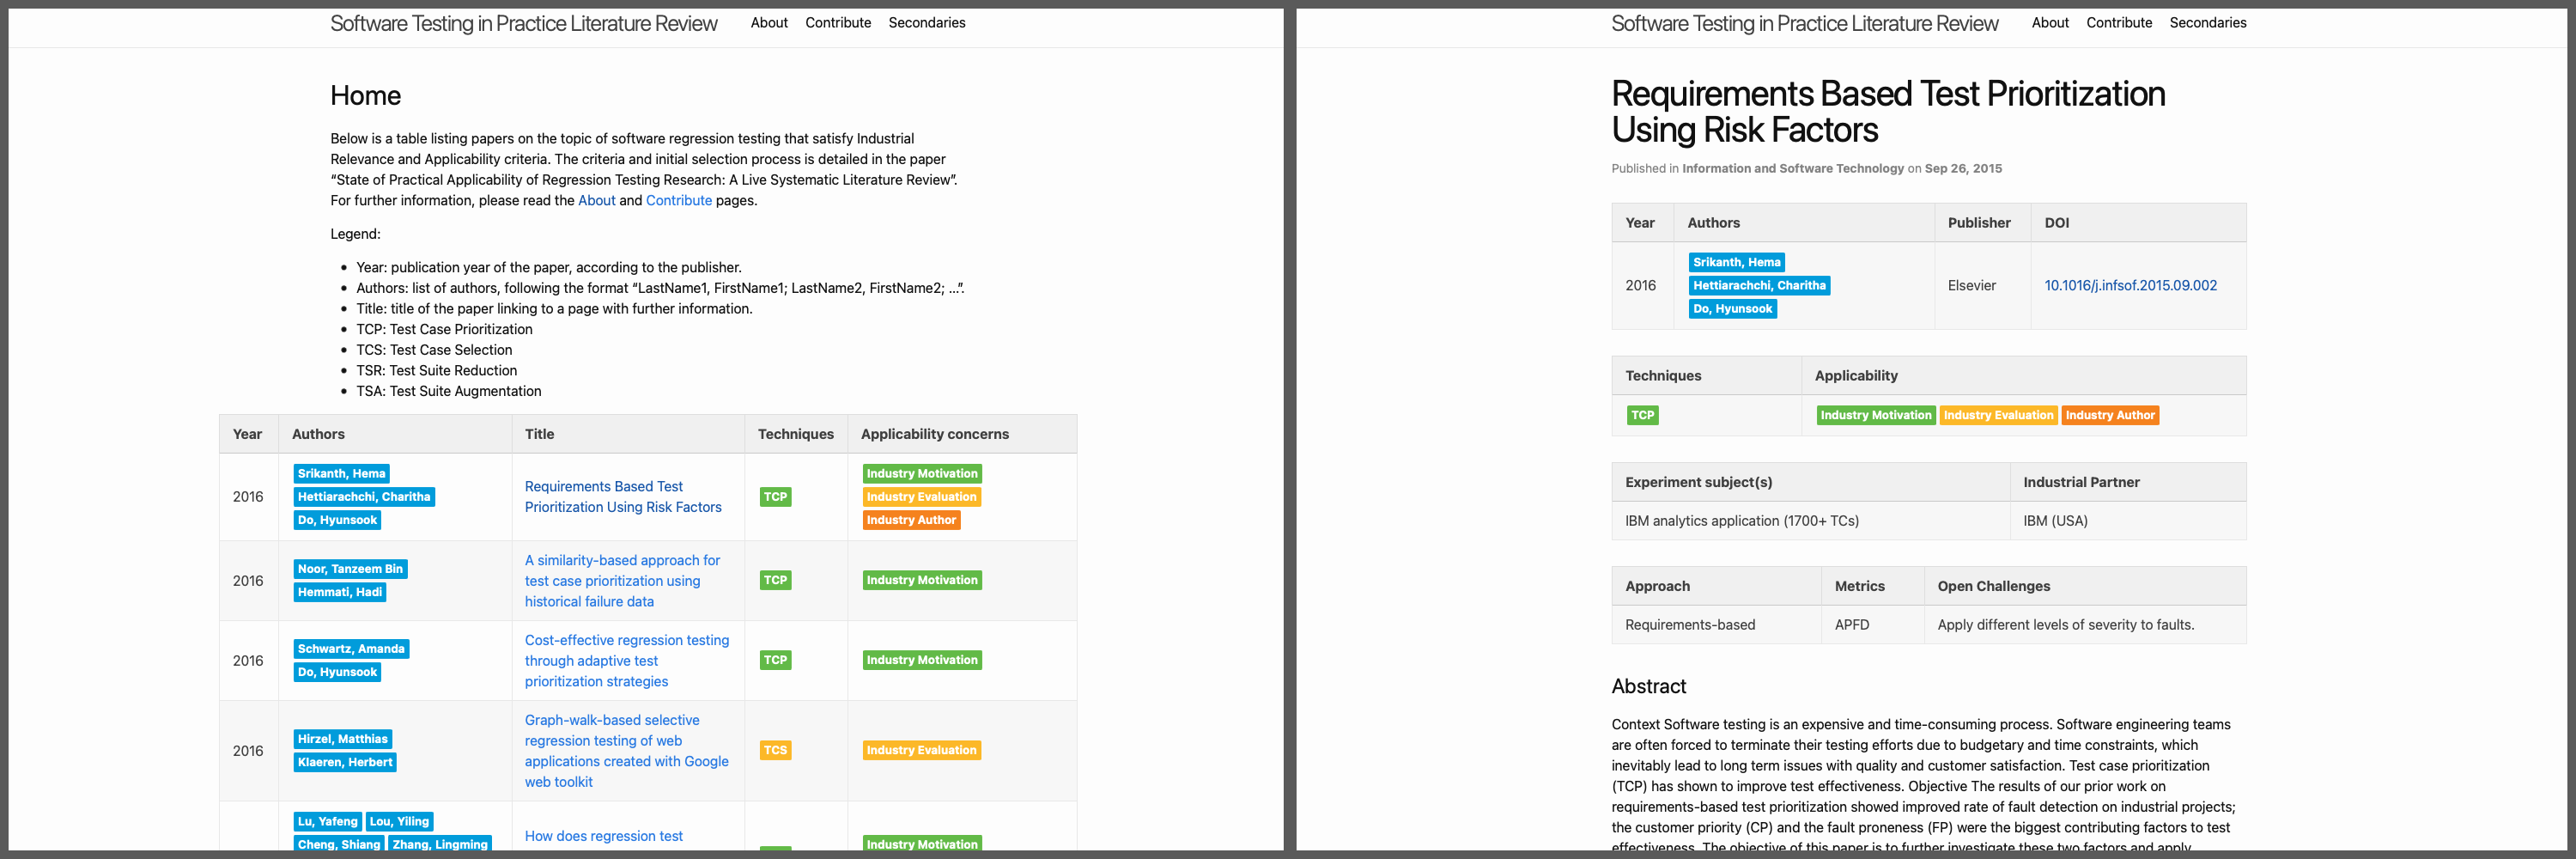
\includegraphics[width=\linewidth]{figures/live_repository_screenshots_4.png}
  \caption{Screenshots from the live repository. From left to right: 1) the main page listing the included papers; and 2) a single paper's page (\citetalias{srikanth_requirements_2016} used as example). }
  \label{fig:live_repository}
\end{figure}

\section{Longevity}\label{subsec:live_longevity}
The main challenge is how to keep this repository alive in the long term.
It is unfeasible for us to add a relevant paper to the repository as soon as it is published, so our plan is to update the list in a yearly basis, re-running the query and screening steps detailed in \Cref{sec:lit_methodology}.
That way, we can at least assure the most recent paper included is no more than one year old.
We are also looking into the possibility of getting automatic notifications when a paper that satisfies certain criteria is published in an online library.
For now, this work is done by the original authors of the literature review; according to future necessities, we will appoint other researchers or graduate students to help with the process.
In addition, we also encourage authors to submit their own work by filling a form linked on the website\footnote{Available at: \url{https://forms.gle/CWGjMrxCe1bnKikk8}.}.

Along with adding more papers to the list, whenever possible we will also add additional information about the ones already included.
This can be triggered by a direct contact by one of the authors, some observed update with the state of that piece of research, or by suggestion of an engaged reader.

At some point after a certain number of years, the definitions we selected for including a paper in the repository will likely need be adjusted.
Whenever an author submits a paper, we will use the opportunity to consider whether or not the paper itself is a good fit for the repository, but also if there are new trends that our existing selection process does not account for.
There will eventually be a point in the future when the industry/academia landscape has shifted and this study will no longer be needed.
When that happens, we will discuss the possibility of freezing the repository and stopping further expansions.

Aside from newer papers, it is always possible that we have missed some relevant papers for a variety of reasons, so the live repository is another way of mitigating that risk.
It is impossible to provide a complete and definitive overview of any field, but we believe that a live repository is the closest approximation that can be expected.

%\todo{we want to keep the information summarized for future researchers/practitioners to gather data}

%\todo{we want to keep it updated as to not need another systematic literature review on the same topic}